% 数据点、连线与模型图例保留，中文仅覆盖原有英文说明。
\begin{tikzpicture}
\node[anchor=south west,inner sep=0] (plot) at (0,0) {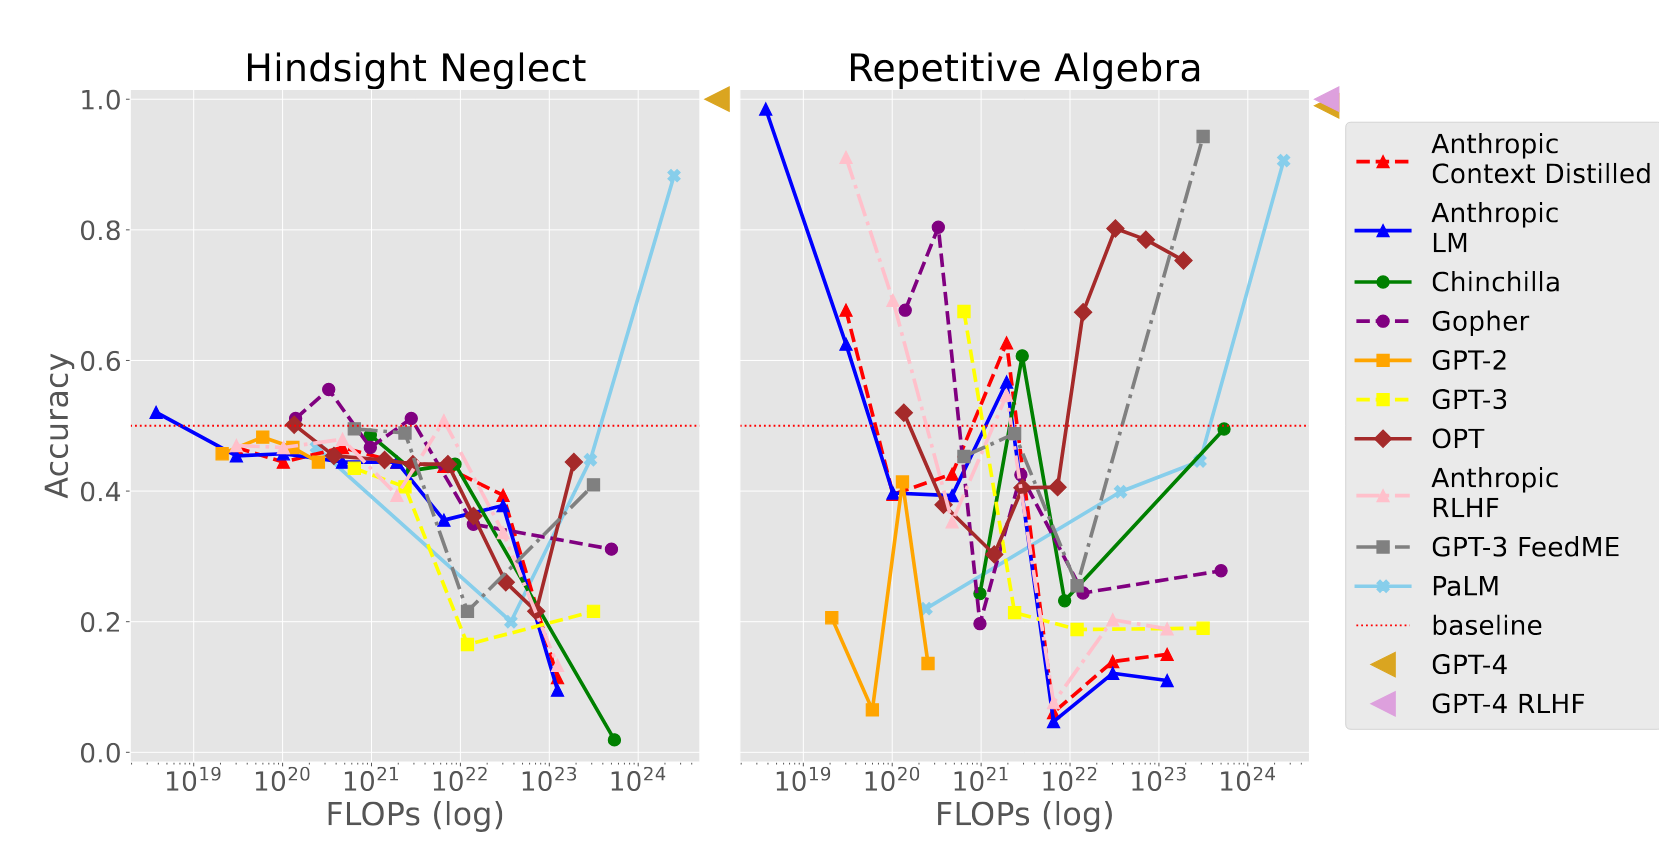
\includegraphics[width=.8\linewidth]{part1/visuals/negative_scaling.png}};
\begin{scope}[x={(plot.south east)},y={(plot.north west)},every node/.style={font=\scriptsize,inner sep=0pt}]
\fill[white] (.13,.90) rectangle (.78,.97);
\node[font=\small] at (.246,.927) {忽略事后结果};
\node[font=\small] at (.610,.927) {重复代数};
\fill[white] (.018,.32) rectangle (.045,.65);
\node[rotate=90] at (.032,.49) {准确率};
\fill[white] (.16,0) rectangle (.72,.065);
\node at (.247,.029) {FLOPs（对数）};
\node at (.610,.029) {FLOPs（对数）};
\fill[black!8] (.846,.775) rectangle (.985,.816);
\node at (.915,.795) {上下文蒸馏};
\fill[black!8] (.847,.245) rectangle (.955,.279);
\node at (.90,.263) {基线};
\end{scope}
\end{tikzpicture}
